\chapter{Conclusions and Recommendations
\label{chap:11}}

% Introduction: Big picture issues

Underground mine safety can only be improved by the addition of technology which increases both safety and 
productivity. By enabling real time measurement of rock cutting forces, the sensor proposed in this work
could improve safety and productivity by allowing machine operators to make decisions in real time without delaying
the machine operation. This will result in more efficient tool use and lead to reduced time lost from accidents.

Technology is used to improve every aspect of mine operation when possible, evidenced by the large body of 
research across many domains of mine operation \cite{LIU202412}.
Much of the current research focusses on wireless transmission and localization systems \cite{9536741, RayChowdhury2021}.
Other novel technology to improve miner safety and productivity even extends to smart helmets \cite{Sharma2018},
used to augment miner senses with real time information from on board sensors.
A very promising technology in the underground mine sector is chipless radio frequency identification, also known as RFID, which uses changes
in capacitance and environmental factors to alter the resonant frequency of a passive antenna \cite{10081221}.
This type of technology would improve the design further by eliminating the requirement local power and computation.

It has long been known that rock cutting forces could be used to infer rock material type or tool wear levels 
if the material and tool condition was known. 
One of the primary contributions of this work is validation of the hypothesis that tool wear and rock type can be 
classified using objective differences in vibrational frequency excitation \cite{Oltmanns24, oltmanns2023low}.
This work shows that the forces themselves are not strictly needed to make this type of classification. 
Different rock types and tool wear conditions will excite characteristic frequencies in the cutting machinery and environment.
This type of analysis has previously been applied to measurement while drilling, also known as MWD, sytems \cite{LIU202412}, 
but not for force measurements directly from the conical pick. 

The \textit{a-priori} estimation of cutting forces from tool parameters and rock properties has been 
investigated extensively, as an estimate of the expected cutting force is needed for initial tool design \cite{Li2018ATM, Morshedlou2023}.
Other efforts to measure forces for conical picks have used custom blocks with strain gauges \cite{s23239521}, 
or bulky experimental equipment in laboratory conditions \cite{WANG2018210}.
This work is the first to use capacitive load cells for force sensing for conical picks. 
These types of load cells are robust to outside interference, can tolerate large forces,
require very little power to operate, and can be made for very low cost compared to the rest of the tooling and other solutions.
Tools lose mass and efficiency as they wear \cite{Pawlik2022-cj}, so accurate tracking of forces during cutting requires a direct sensor.

Broader impacts of this technology are increased safety for underground miners 
and advancement of rock cutting load cell technology.
Miner safety would be improved by allowing them to perform their role from a greater distance.
Rock cutting load cell technology has been advanced by this study, 
as no prior load cells using capacitive technology have been published for conical picks.
These innovations are the result of years of methodical developments across many domains.

\subsection{Summary of Methods and Materials}

In the begining of the development of the load cell, detailed in Chapter~\ref{chap:P1},
the meaurement results were very nonlinear. However, the frequency response of the sensor
was still correlated with the frequency response of the different materials and tool wear conditions.
This phenomena was investigated further in Chapter~\ref{chap:P2}, using acoustic data for tool wear classification.
At the end of the development of the load cell in this work, shown in Chapter~\ref{chap:P3},
measurements with much greater linearity were achieved by optimizing the sensor parameters.

The materials used to test the capacitive load cell were concrete, limestone, and coal.
The material used to test tool wear classification via acoustic signals was concrete.
Tool wear and material classification were done with the capacitive load cell using a concrete and limestone sample.
Force measurement with the capacitive load cell was done using two coal samples.
The different samples are shown in \ref{fig:samples}.

\begin{figure}[ht]
\centering
\includegraphics[width=2.0in]{ch9_concrete.jpg}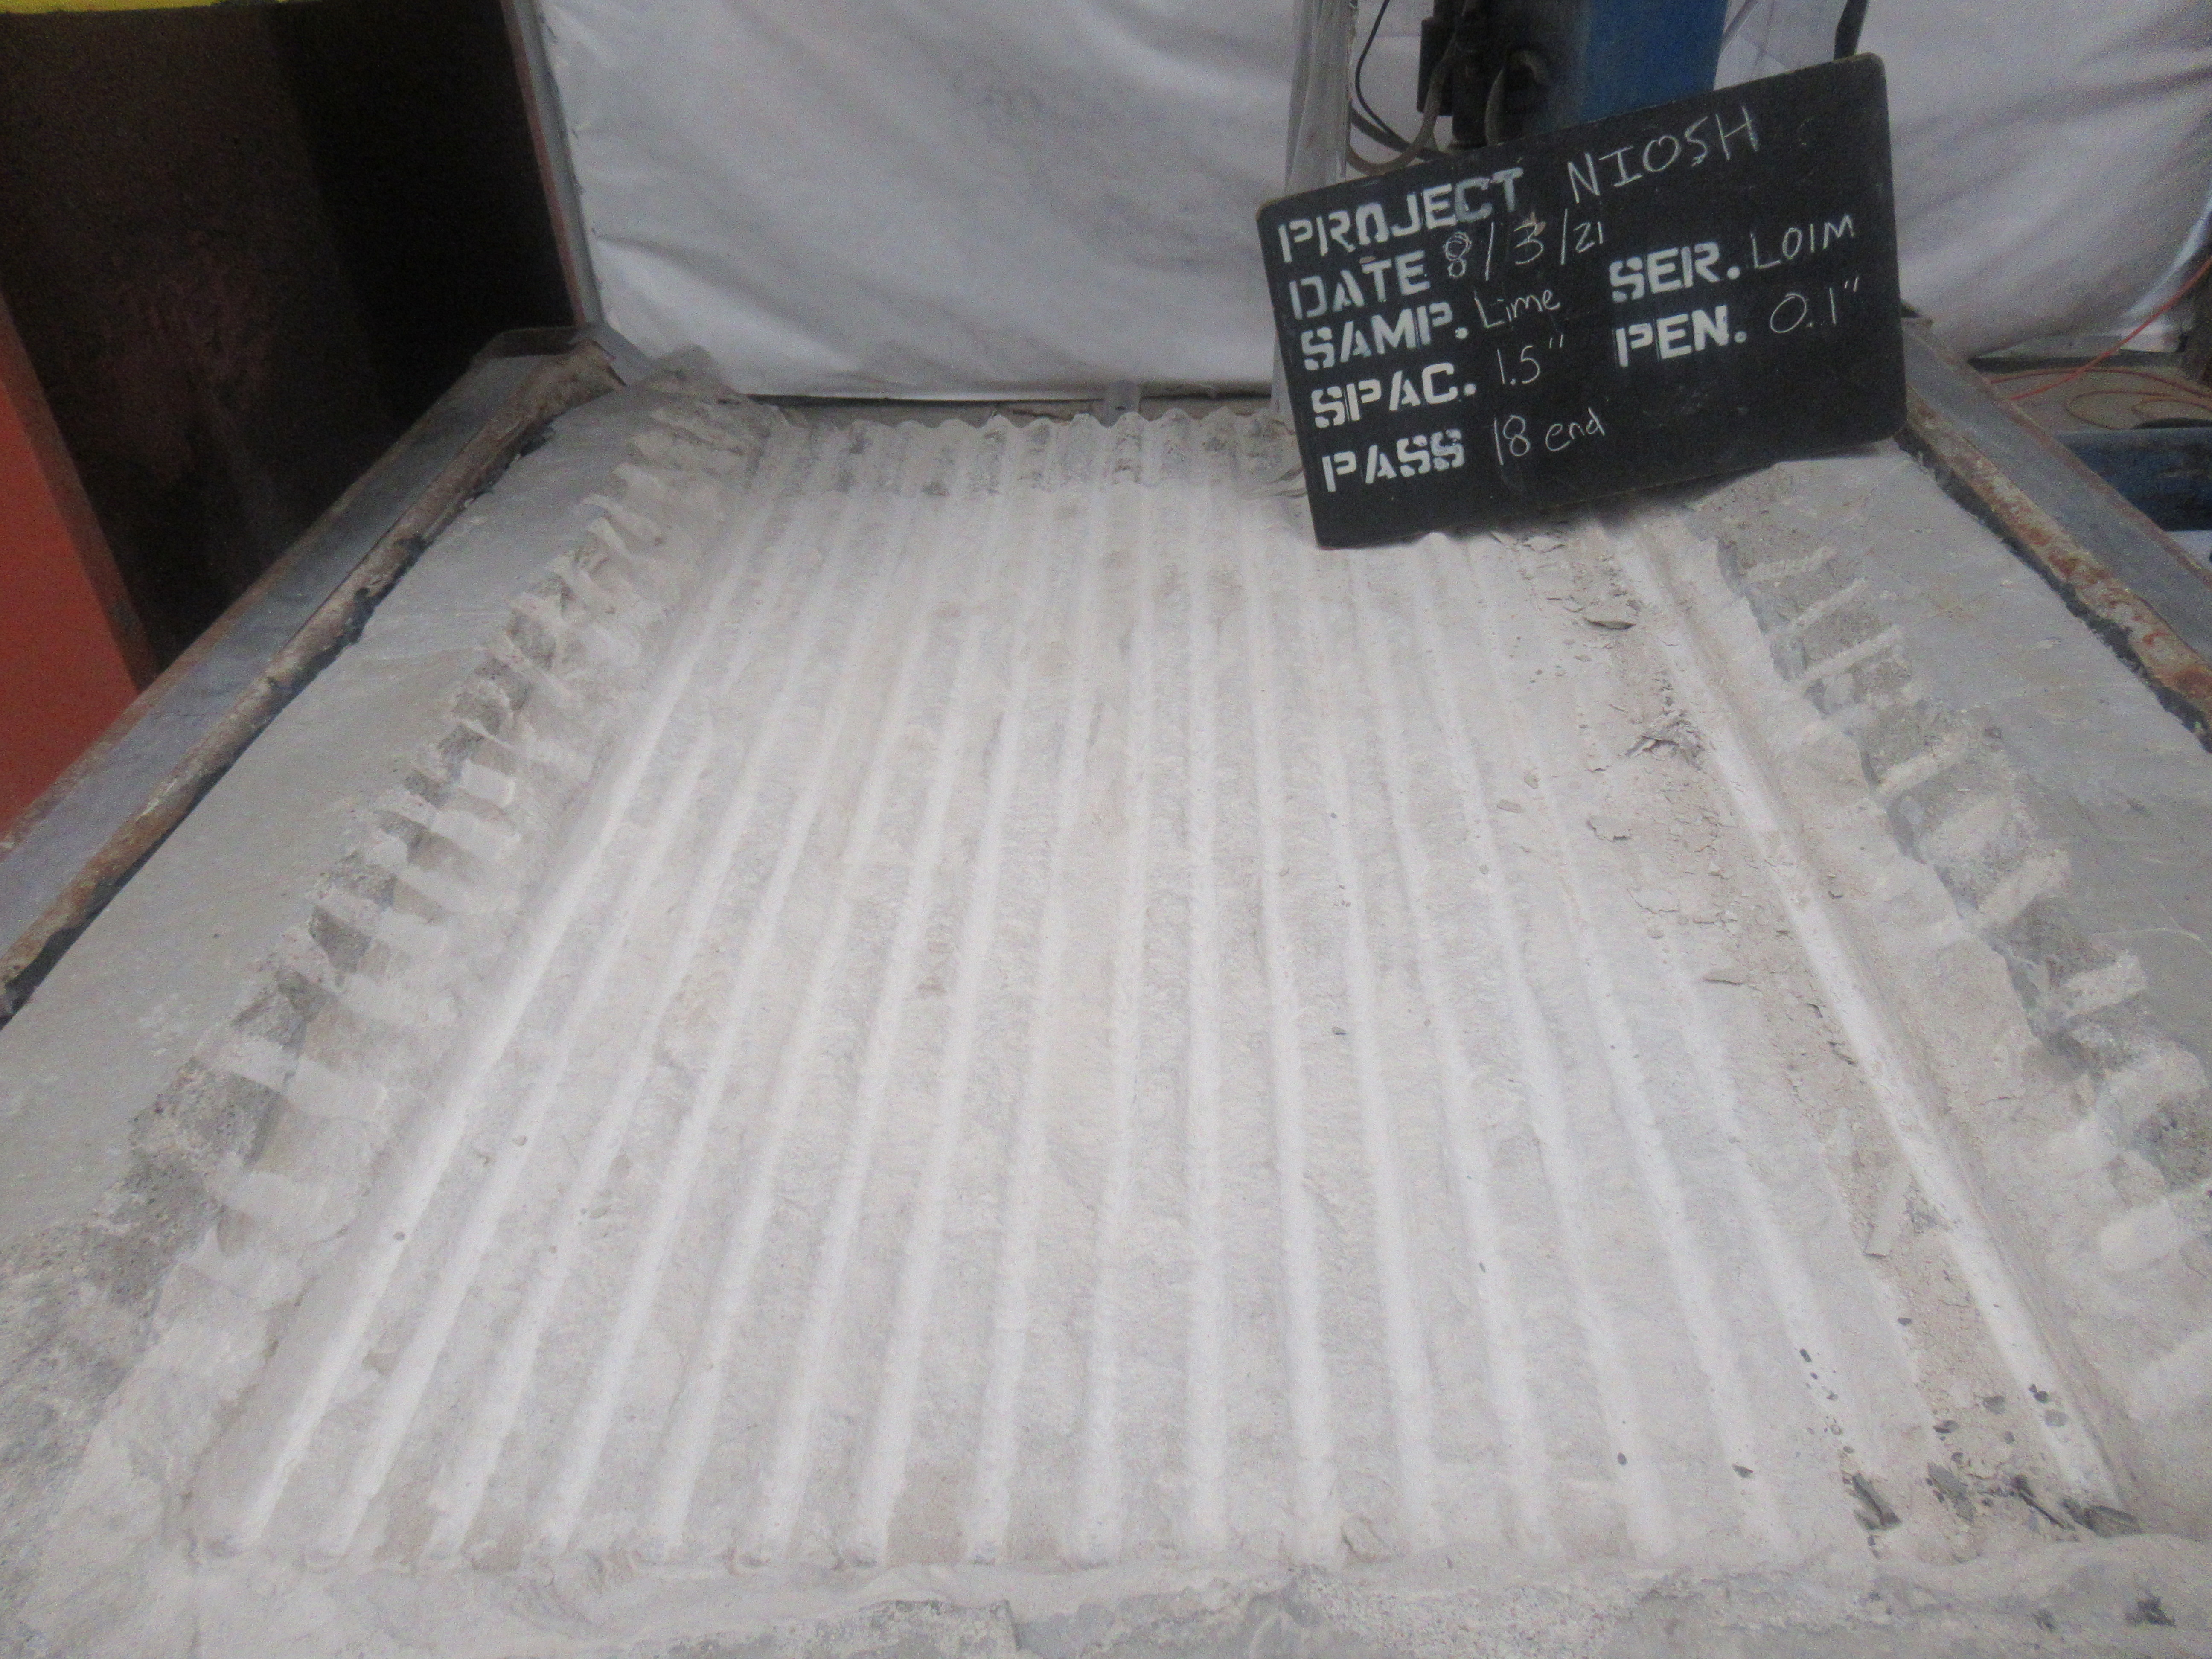
\includegraphics[width=2.0in]{ch9_limestone.jpg}\includegraphics[width=2.0in]{ch9_coal2.jpg}
\caption{
From left to right: concrete sample, limestone sample, and one of the coal samples in the Linear Cutting Machine box.
}
\label{fig:samples}
\end{figure}

For both works involving the capacitive load cell, the same measurment setup was used.
The measurement setup for the capacitive load cell during the rock cutting experiments in shown in \ref{fig:datalogsetup}.
The figure shows a laptop computer connected via USB to a microcontroller which interfaces with
the capacitance to digital converter over I$^2$C to read the sensor. The system is powered over the USB connection only.
The acoustic measurement setup was similar, expect instead of the custom measurement system, an off the shelf 
microphone was plugged into the USB port. The general methods for classification were the same between 
Ch.~\ref{chap:P1} and Ch.~\ref{chap:P2}. In Ch.~\ref{chap:P3} regression was used to model force measurements.
\begin{figure}[ht]
\centering
\includegraphics[width=4.5in]{ch9_datalogsetup.png}
\caption{
The setup of the experimental data collection system.
}
\label{fig:datalogsetup}
\end{figure}

The ultimate aim of this research was to produce a force sensor capable of measuring rock cutting forces. 
This was achieved using a capacitive load cell with mostly linear dynamics. It was necessary to iterate the design
a few times to find a configuration that was linear enough. The sensor model was still aided by using nonlinear modeling.
The sensor in this work was designed to fit a force input range of 0 to 200 kN.
Over this range, it was desired to have at least 10 discrete values, such as increments of 20 kN.
The bandwidth was limited by the capacitance to digital converter, 
which read each channel at a rate of around 400 Hz. The nominal resonant frequency of the sensor 
was around 2 MHz. The max strain for the design was set to 10\% of the thickness, this was to
minimize fatigue on the case and to preserve linear model assumptions.

\subsection{Summary of Results}

% Comparison of classification results
The tool wear classification results for Chapter~\ref{chap:P1} and Chapter~\ref{chap:P2} can be compared 
on the basis of their confusion matrices. The capacitive load cell showed very little confusion between the tool wear
categories, achieving perfect classification of the \textit{new} tools in the study and very little confusion elsewhere.
The acoustic sensor on the other hand had a small but significant amount of confusion between all categories.
This demonstrates the superiority of direct sensing of the cutting forces over indirect observation regarding classification accuracy.

% Comparison of force measurement results
The linear force measurement ability of the different sensor designs is shown in detail in \ref{compare1} and \ref{compare2}.
The key point of comparison from \ref{compare1} is the large increase in linearity and comparable sensitivity 
when observing the improvements of the updated sensor design. During the rock cutting testing, discussed in \ref{compare2},
the main point is that the first sensor design was very insensitive during rock cutting, while the updated design had
much greater sensitivity in the rock cutting scenario. The thick polyimide coating around the thin sensing region
in the first design inhibited force transfer to the sensing region. In the updated design, the polyimide layer
outside the sensing region was much smaller.

% Tables of links to code and data
The code and data for this study are available to the public on the internet. 
The links for each work are summarized below in \ref{tab:links}.
The results for each work can be reproduced from the data by running the appropiate script in the linked repositories.
The firmware for the measurement system and the corresponding computer program are also available, and linked in \ref{tab:links}.
These links are shared so that this work can easily be verified, and so that the methods can be easily adapted for other research tasks.

\begin{table}[]
\centering
\caption{Links to the code and data for experiments}
\label{tab:links}
\begin{tabular}{|r|l|}
\hline
Work                                                  & Link \\ \hline
Frequency based rock and wear classification & \url{github.com/Fworg64/limestone_experiment}     \\ \hline
Frequency based acoustic wear classification     &  \url{github.com/Fworg64/concrete_tool_wear}    \\ \hline
Force measurement using capacitive load cell          &  \url{github.com/Fworg64/air_gap_coal_sensor_model}    \\ \hline
Firmware for measurement microcontroller       &  \url{github.com/Fworg64/DAQuery}    \\ \hline
Computer software for measurement capture             &  \url{github.com/Fworg64/reDAQ}    \\ \hline
\end{tabular}
\end{table}

A summary of numerical metrics for each study is shown in \ref{tab:results}.
The dynamic capcitive load cell from Ch.~\ref{chap:P1} is able to reliably classify 
rock type and tool wear using frequency measurements collected directly from the tool.
The acoustic tool wear classification method gets a similar score over its dataset 
when compared to the results of the capacitive sensor over its dataset.
These scores cannot be compared directly due to the differences in experimental setup, 
but they both show that either method could be used with expectations for success.
Regarding sensor sensitivity, the iterated capacitive sensor design was able 
to improve both sensitivity and linearity, as the 2nd design could be used
to generate force measurements, while the 1st design was too nonlinear for this purpose.
The 2nd design was over twice as sensitive when compared to the first design.



\begin{table}[]
\centering
\caption{Links to the code and data for experiments}
\label{tab:results}
\begin{tabular}{|r|r|c|}
\hline
Application                                                  & Metric & Value \\ \hline
Frequency based rock classification with cap. sensor & F1 Score & 0.831 $\pm$ 0.085 \\ \hline 
Frequency based wear classification with cap. sensor & F1 Score & 0.950 $\pm$ 0.004 \\ \hline
Frequency based wear classification with acoustic sensor& F1 Score & 0.900 $\pm$ 0.020 \\ \hline
Sensitivity of 1st cap. sensor in rock cutting & Ticks/kN &  $\approx$ 1 \\ \hline
Sensitivity of 2nd cap. sensor in rock cutting & Ticks/kN & $\approx$ 2.7\\ \hline
\end{tabular}
\end{table}


\subsection{Discussion}

This work investigated using frequency data for classification in rock cutting,
which proved to be a functional means of identifying both tool wear and material type.
Based on the results in this work from the tool wear and rock material type classification, shown in Ch.~\ref{chap:P1}, 
and acoustic tool wear classification, shown in Ch.~\ref{chap:P2}, high frequency classification 
should also be considered a valid method for determining material type and tool wear. 

The original goal of this research was to develop a load cell capable of measuring cutting forces.
The first design did not meet this requirement, but it was found that the recorded measurements'
frequency content still varied according to material type and tool wear conditions.
The initial design was not adequately modeled by linear components, but still 
had a consistent response in the frequency domain for different conditions.
This type of sensor is a dynamic sensor, which means that its response
is largely influenced by its dynamics. For the first sensor design,
these dynamics filter and compress the vibrations while still providing enough information for classification.

Using the cutting tool to protect the sensor while it measures vibrations or cutting forces,
the sensor was placed behind the sleeve for a balance of protecting the sensing element 
and providing proximity to the cutting forces to be measured.
Integrating the sensor with the conical pick would facilitate easy replacement of the sensor when the pick is replaced,
but likely cause more sensors to be consumed due to the greater proximity to the cutting interface.
Optimal placement of the sensor will require future testing and validation.

This work has contributed to the modeling and use cases for capacitive load cells. 
In Ch.~\ref{chap:P3}, equations for the
closed gap sensor are developed, which show that the sensor sensitivity approaches infinity as the force increases.
This relationship works well in the rock cutting domain, as the presence of large forces is interesting
in both rock type and tool wear classification. 
This relationship offsets the insensitivity of the tough sensor design, 
allowing a robust and linear sensor to be sensitive as well.
The dynamics of a capacitive sensor in this application will 
naturally boost these peaks in force while reducing the sensitivity to smaller forces. This makes
detection of the large forces easier.

\subsubsection{Recommendations}

\begin{enumerate}

\item The sensor linearity could be improved by optimizing the film thickness and the number of electrodes.
A simple way to improve the sensitivity of this sensor design would be to stack alternating electrodes and polyimide layers.
Each additional layer increases the sensitivity by increasing the capacitance and reducing the overall stiffness.
A suitable layer height for good deformation characteristics could be stacked to produce a squishier, but more sensitive sensor.

\item Directly embedding a piezo element within the tool could
also serve to measure higher frequency vibrations which vary with cutting parameters.
Another use for piezo elements in the sensor would be local power generation for the sensor. 
A sensor which could generate its own power from the large forces present would be able to 
eliminate additional wiring from the design. Sensors that generate their own power would be able to 
emit signal wirelessly using the power generated by on-board piezo crystals.

\item To reduce costs for this design, one could integrate the steel case with the body of the cutting tool.
It would be possible to create a channel for the sensing element in either the block or the sleeve, and then
when the cutting system is assembled, these two components would act as an integrated case for the sensor.
This type of design might increase overall shipping costs if the heavy tools must be sent around and modified before final use.
For this reason, a separate sensor which is lightweight and easy to integrate on-site is desired.

\item A drawback of the presented sensor design is the use of many integrated electronics. These devices are low cost and low power,
but the margins for the sensing device are small when it comes to cost and power. A sensor design which is mostly analogue but
still capable of wireless transmission of information would be more useful than one which requires additional power
and translation equipment. Such a sensor would be the lowest cost design, as it would be a simple design.
Refining the design to this point will take additional development, but is possible.

\end{enumerate}

\subsection{Conclusion}

The impact of the sensor is limited by the distance of its transmission. 
The further the information can reach, the more productivity can be increased for an underground mine.
If the measurements are incorporated to the machine, the machine could have automatic emergency brakes 
implemented to reduce accidental roof cutting. If the measurements are transmitted to operators, the operators
can infer tool wear without stopping operation and also estimate material strength in real time.
If the measurements are sent to an outside office, trends can be analyzed to determine when machine operators
are the most efficient. This type of rock cutting force sensor for conical picks just scratches the surface of these desirable applications.


